\printbibliography
\nocite{*}
\appendix

\begin{changemargin}{-2cm}{-4cm}

\addcontentsline{toc}{chapter}{Scripts Python}
\label{Scripts}
\chapter*{Script principal}
\label{main}
\inputminted[fontsize=\scriptsize, linenos=true]{Python}{../script/main.py}

\chapter*{Script de résolution des sudokus}
\label{resolution}
\inputminted[fontsize=\scriptsize, linenos=true]{Python}{../script/resolution.py}

\chapter*{Script de gestion de la caméra}
\label{camera}
\inputminted[fontsize=\scriptsize, linenos=true]{Python}{../script/camera.py}

\chapter*{Script d'affichage du sudoku}
\label{display}
\inputminted[fontsize=\scriptsize, linenos=true]{Python}{../script/display.py}

\chapter*{Script de gestion des moteurs pas-à-pas}
\label{step_motor}
\inputminted[fontsize=\scriptsize, linenos=true]{Python}{../script/step_motor.py}

\chapter*{Script permettant l'écriture d'un sudoku}
\label{write}
\inputminted[fontsize=\scriptsize, linenos=true]{Python}{../script/write.py}

\addcontentsline{toc}{chapter}{Mises en plan des pièces conçues en 3D}

\chapter*{Mise en plan du chariot}

\begin{figure}[!h]
\label{chariot}
 \center
 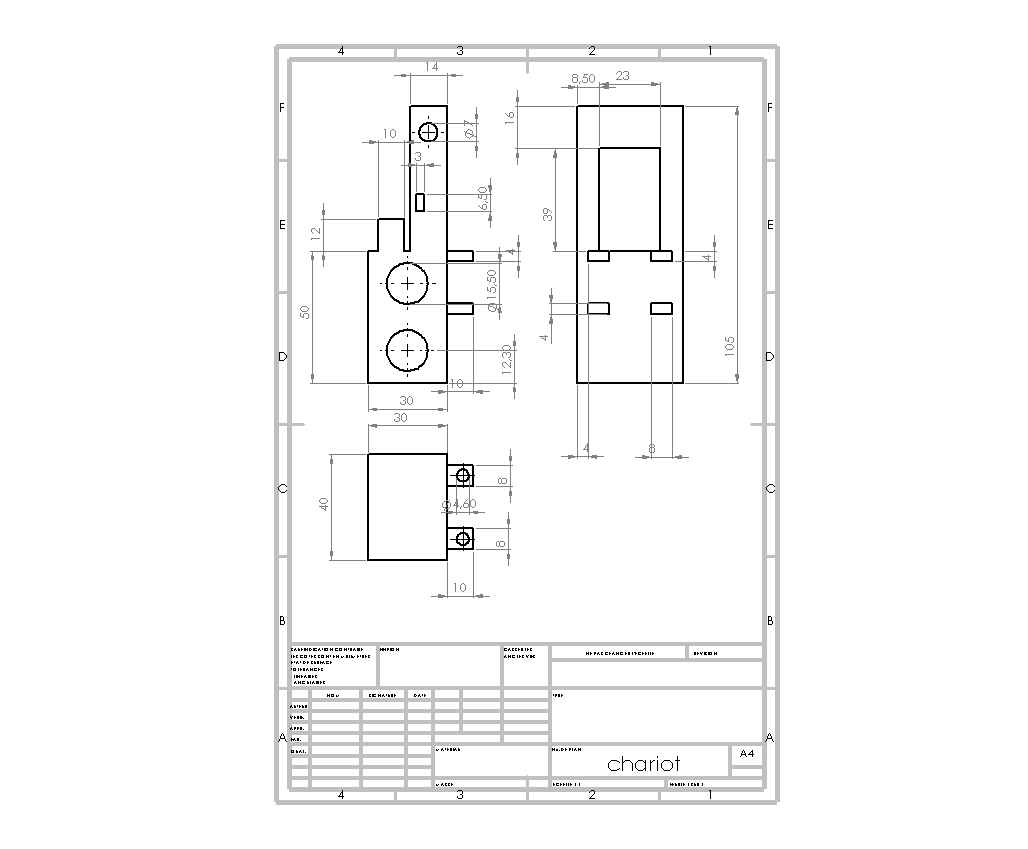
\includegraphics[scale=1]{../3Dmodels/chariot.png}
\end{figure}

\chapter*{Mise en plan du support du stylo}
\begin{figure}[!h]
\label{supportstylo}
 \center
 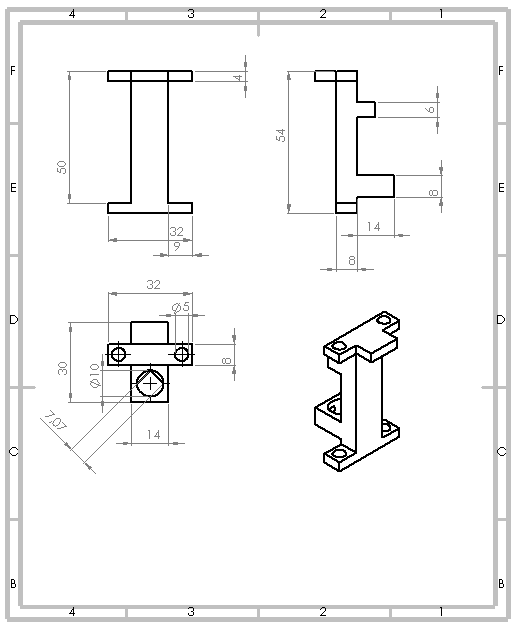
\includegraphics[scale=1]{../3Dmodels/supportstylo.png}
\end{figure}

\chapter*{Mise en plan du lien chariot/caméra}
\begin{figure}[!h]
\label{chariotcamera}
 \center
 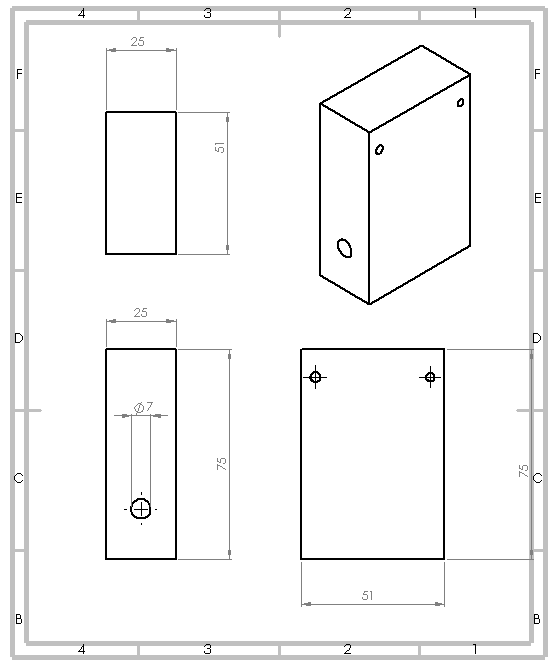
\includegraphics[scale=0.95]{../3Dmodels/camerachariot.png}
\end{figure}

\chapter*{Mise en plan du support de la caméra}
\begin{figure}[!h]
\label{supportcamera}
 \center
 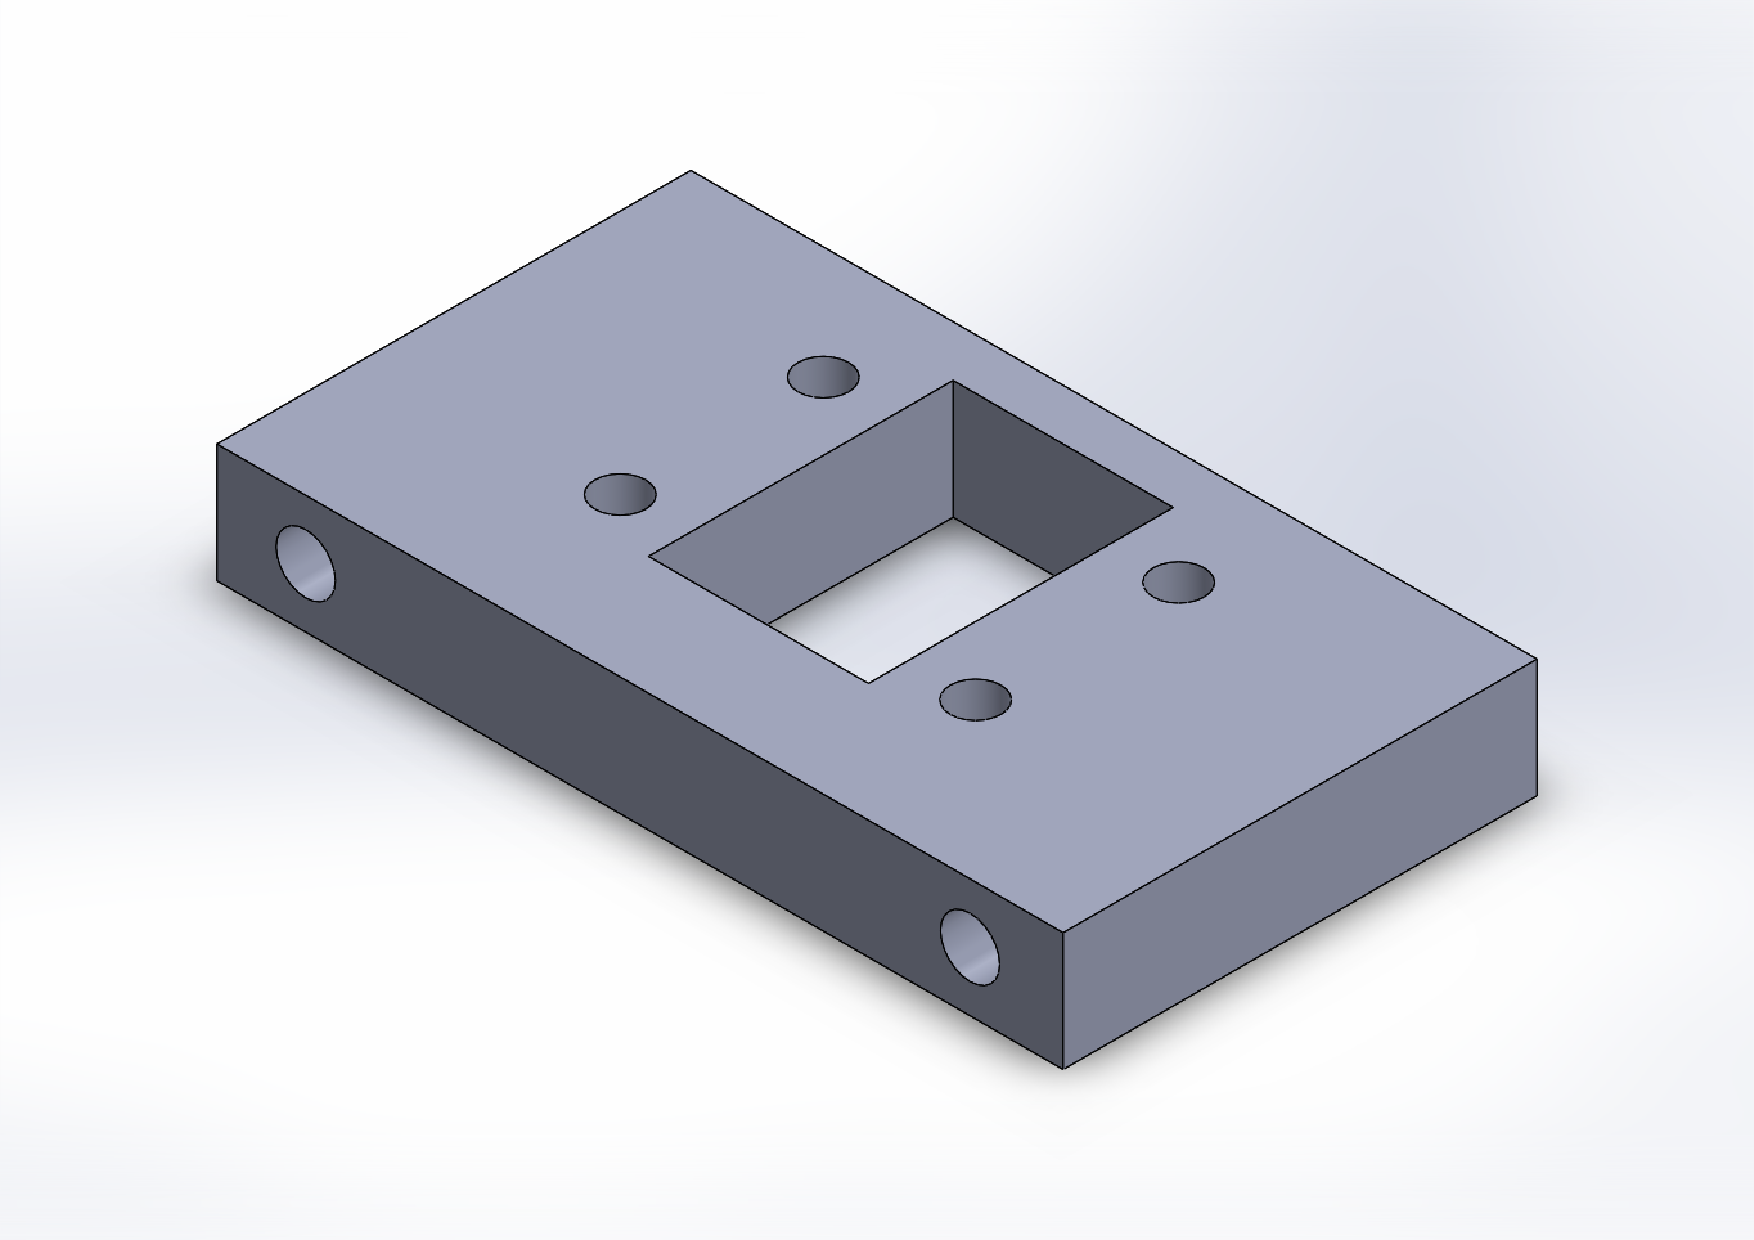
\includegraphics[scale=0.95]{../3Dmodels/camera.png}
\end{figure}

\end{changemargin}